\providecommand{\main}{../../..}
\documentclass[\main/dresen_thesis.tex]{subfiles}
  \renewcommand{\thisPath}{\main/chapters/monolayers/intro}

\begin{document}
  A primary goal of this work is the study of magnetic dipolar interactions between nanoparticles.
  Due to the highly directional nature of dipolar magnetism, random orientation of the nanoparticles and random packing, as described in the previous chapter, cloud the observation of macroscopic effects arising from the interaction.
  Therefore an intermediate goal towards the observation of dipolar interaction is the successful preparation of highly ordered nanostructures.
  Simple arrangements that have been discussed extensively in theory, are the square lattice and hexagonal lattice in the plane.
  Here, dipolar coupling leads to an emergent macroscopic states for the nanostructure, namely a super antiferromagnetic state for the square lattice and a super ferromagnetic state for the hexagonal lattice \cite{Politi_2002_Dipol, Russier_2001_Calcu, Varon_2013_Dipol}.
  In this work, a procedure to fabricate such long range ordered nanostructures from nanocubes and nanospheres has been developed.
  The preparation of such self-assembled lattices with long-range order is presented in detail on the case of the square lattice from cobalt ferrite nanocubes in this chapter.
  For this purpose this chapter separates into multiple parts, the synthesis following protocols from literature and characterization of magnetic cobalt ferrite nanocubes is described first, and subsequently the production of monolayer samples from same nanoparticles is described.
  For selected nanoparticles and monolayers, the quantitative evaluation of the structures are shown, as well as the characterization of their magnetic properties. Emergent magnetic properties that are not observed for the individual nanoparticles are described and compared to model calculations.
  \\

  Cobalt ferrite nanoparticles are nowadays routinely synthesized following methods such as co-precipitation \cite{Fried_2001_Order}, sol-gel \cite{Niederberger_2009_Metal}, micro emulsions \cite{Pillai_1996_Synth}, or thermal decomposition.
  For thermal decomposition, one can further differentiate between hot-injection \cite{Hyeon_2003_Chemi} and heating up methods \cite{Embden_2015_TheHe}.
  Where the first promises monodisperse nanoparticles by keeping the nucleation time period of the synthesis short, the latter is especially promising in being scaleable and highly controllable \cite{Park_2004_Ultra}.
  The heating up method is used extensively in this work to synthesize nanocubes and nanospheres of cobalt ferrite and iron oxide and is further elaborated in the following.

  A popular heating up route to synthesize nanoparticles is to first prepare a metal oleate precursor from metal salts, which is subsequently slowly heated above it's decomposition temperature in a high-boiling solvent, where it is aged in the presence of oleic acid and additional reagents to direct the growth and shape \cite{Park_2004_Ultra, Wetterskog_2014_Preci}.
  For example, the shape of cobalt ferrite nanoparticles can be tuned by adding sodium oleate as precursor before the heating up process \cite{Bodnarchuk_2009_Excha}.
  The sodium oleate attaches to the (100) facets of forming nanocrystals and fosters the growth along the [111] direction of the crystal \cite{Bodnarchuk_2009_Excha}.
  By tuning the ratio of sodium oleate to the oleate precursor and adjusting the aging time, this process allows to prepare either nanospheres, nanocubes, polyhedral nanoparticles or even star-like nanoparticles \cite{Bodnarchuk_2009_Excha, Bao_2009_Forma, Wetterskog_2014_Preci}.

  Wetterskog \etal extensively studied the formation of maghemite nanospheres and nanocubes, following the same route for iron oleate in the synthesis \cite{Wetterskog_2014_Preci, Wetterskog_2013_Anoma}, and found multiple deviations from the expected pure phase for the nanoparticles.
  For one, during the oleate synthesis \ch{CO} is constantly being produced from the solvents leading to an reaction environment where \ch{Fe^{3+}} is reduced to \ch{Fe^{2+}} \cite{Hai_2010_Sizec}.
  Therefore, in the synthesis a w\"ustite core is formed and only by post-synthesis oxidation a maghemite shell is obtained \cite{Wetterskog_2013_Anoma}.
  On the other hand, a defect structure can be observed in the nanoparticles.
  Even though the nanoparticle magnetization can be enhanced by forced oxidation at elevated temperatures of $150^\circ$ after the synthesis, anti-phase boundaries remain after complete oxidation of the particles \cite{Wetterskog_2013_Anoma} and the defective structures across the nanoparticle volume correlates with a lower degree of magnetism in comparison to bulk material.
  Additionally it is observed, if the particles are aged for too long, the oleic acid shell degrades and the nanoparticles become unstable in dispersion \cite{Wetterskog_2013_Anoma}.
  The same observations of a core-shell structure are also made in literature for the synthesis of cobalt ferrite nanoparticles from metal oleates \cite{Bodnarchuk_2009_Excha}.
  Here however, cobalt ferrite provides a higher oxygen diffusion barrier and it is technically harder to oxidize cobalt ferrite nanoparticles completely \cite{Chen_2015_Synth}.
  Chen \etal \cite{Chen_2015_Synth} showed that after $120 \unit{days}$ only a $2 \unit{nm}$ oxidized shell is observed for $12.5 \unit{nm}$ and $19 \unit{nm}$ sized nanospheres and only after adding dehydrated trimethylamine N-oxide (TMNO) to the as-prepared cobalt ferrite nanoparticles with subsequent aging of the particles for over $20 \unit{h}$, a shell of $4 \unit{nm}$ can be oxidized until the oxygen barrier from cobalt ferrite stops any further oxidation.

  An alternative popular heating up synthesis is achieved by the thermal decomposition of cobalt and iron acetylacetonates in a high boiling solvent such as dibenzyl ether with the presence of oleic acid or oleylamine \cite{Sun_2002_SizeC, Wu_2014_Monol}.
  Again, the addition of sodium oleate leads to the formation of nanocubes, such as in the oleate synthesis route, when the amount is tuned to the oleic acid content and aging time \cite{Wu_2014_Monol}.
  During the acetylacetonate route, no reducing carbon monoxide is formed, however it has to be noted that from the decomposition of the acetylacetonates, acetone and carbon dioxide is constantly being produced \cite{Lu_2015_Synth}
  \begin{align}
    \ch{Co(acac)_2} + \ch{Fe(acac)_3} \rightarrow \ch{CoFe2O4} + \ch{CH3COCH3} + \ch{CO2}.
  \end{align}
  And indeed, x-ray diffraction of particles by acetylacetonates shows an agreement with the crystal structure of \ch{CoFe2O4} \cite{Wu_2014_Monol, Sathya_2016_Cofeo} and elemental mapping further confirms the homogeneous distribution of cobalt and iron inside the particle \cite{Sathya_2016_Cofeo}.
  The ratio of cobalt to iron in the nanoparticle is observed to be lower than the feed ratio of the synthesis meaning that not all of the cobalt acetylacetonate is converted to the nanoparticles and part remains in solution, leading to a composition of \ch{Co_x Fe_y O_4}, however the ratio can tuned towards \ch{CoFe2O4} by starting from a higher feed ratio  \cite{Sathya_2016_Cofeo, Yu_2013_Cobal, Wu_2014_Monol}.
  Using M\"ossbauer spectroscopy, the observation of two sub-spectra with an isomer shift below $\mathrm{IS} < 0.4 \unit{mm/s}$ \cite{Pianciola_2014_Sizea}, for cobalt ferrite particles which are synthesized from acetylacetonates, shows that no \ch{Fe^{2+}} is present but that all iron is in a \ch{Fe^{3+}} state, distributed on the A and B sites of the inverse spinell \cite{Angotzi_2017_Spine, Figuera_2015_Moess}.

  Particles in the size range of $10 \ldots 20 \unit{nm}$ obtained by the acetylacetonate route, show strong magnetic properties such as a coercivity in the order of $2 \unit{T}$ at $10 \unit{K}$ \cite{Sun_2002_SizeC, Sathya_2016_Cofeo} and a saturation magnetization in the order of $230 \ldots 300 \unit{kA m^{-1}}$ \cite{Wu_2014_Monol, Sathya_2016_Cofeo}.
  The homogeneous composition and strong magnetic properties therefore make these particles good candidates for the case study of magnetic interparticle interactions.
  \\

  Once the nanoparticles are prepared and available stable in dispersion, multiple methods are known in literature to prepare monolayers on a substrate starting from a nanoparticle dispersion.
  Among the most prominent techniques are the Langmuir-Blodgett/Schaefer method \cite{Ukleev_2017_Selfa, Pauly_2011_Monol, Fried_2001_Order}, spin-coating \cite{Mishra_2012_Selfa}, doctor blade casting \cite{Bodnarchuk_2010_Large}, dip coating \cite{Kim_2002_Multi} and drop casting \cite{Bigioni_2006_Kinet}.
  Depending on the applied technique, the resulting order of the nanoparticles can vary greatly.
  While methods as spin-coating and dip-coating are quick to perform, the in-plane order of the particles is comparably poor to results obtained from evaporation-driven processes that allow for a slow self-assembly process of the particles.

  The Langmuir-Blodgett/Schaefer technique is a method that was designed for the formation of monolayers of organic molecules, but has been transferred to the study of nanoparticle monolayer formation \cite{Heitsch_2010_Gisax, Vorobiev_2015_Subst}.
  Here, the dispersion is allowed to evaporate slowly from an organic solvent on a water surface, where it then is compressed by movable beams on the surface to monolayer density.
  The Langmuir-Blodgett method then proceeds to transfer the particles from the water surface on a wafer by lifting a previously inserted substrate vertically out of the water.
  Whereas the Langmuir-Schaefer method use a wafer with hydrophobic coating as a stamp on the particles to transfer the layer.
  In-situ XRR and GISAXS studies on the water surface show that a high degree of in-plane order on the surface is possible for $10 \unit{nm}$ sized nanoparticles \cite{Vorobiev_2015_Subst}.
  The final experimental challenge is then to transfer the ordered particles from the surface to the wafer without destroying the order.
  A study of Wen \etal \cite{Wen_2011_Ultral} shows that by modification of the Langmuir through, where additionally the solvent evaporation is controlled, micrometer sized ordered arrays can be obtained by the Langmuir-Schaefer method.


  \begin{figure}[tb]
    \centering
    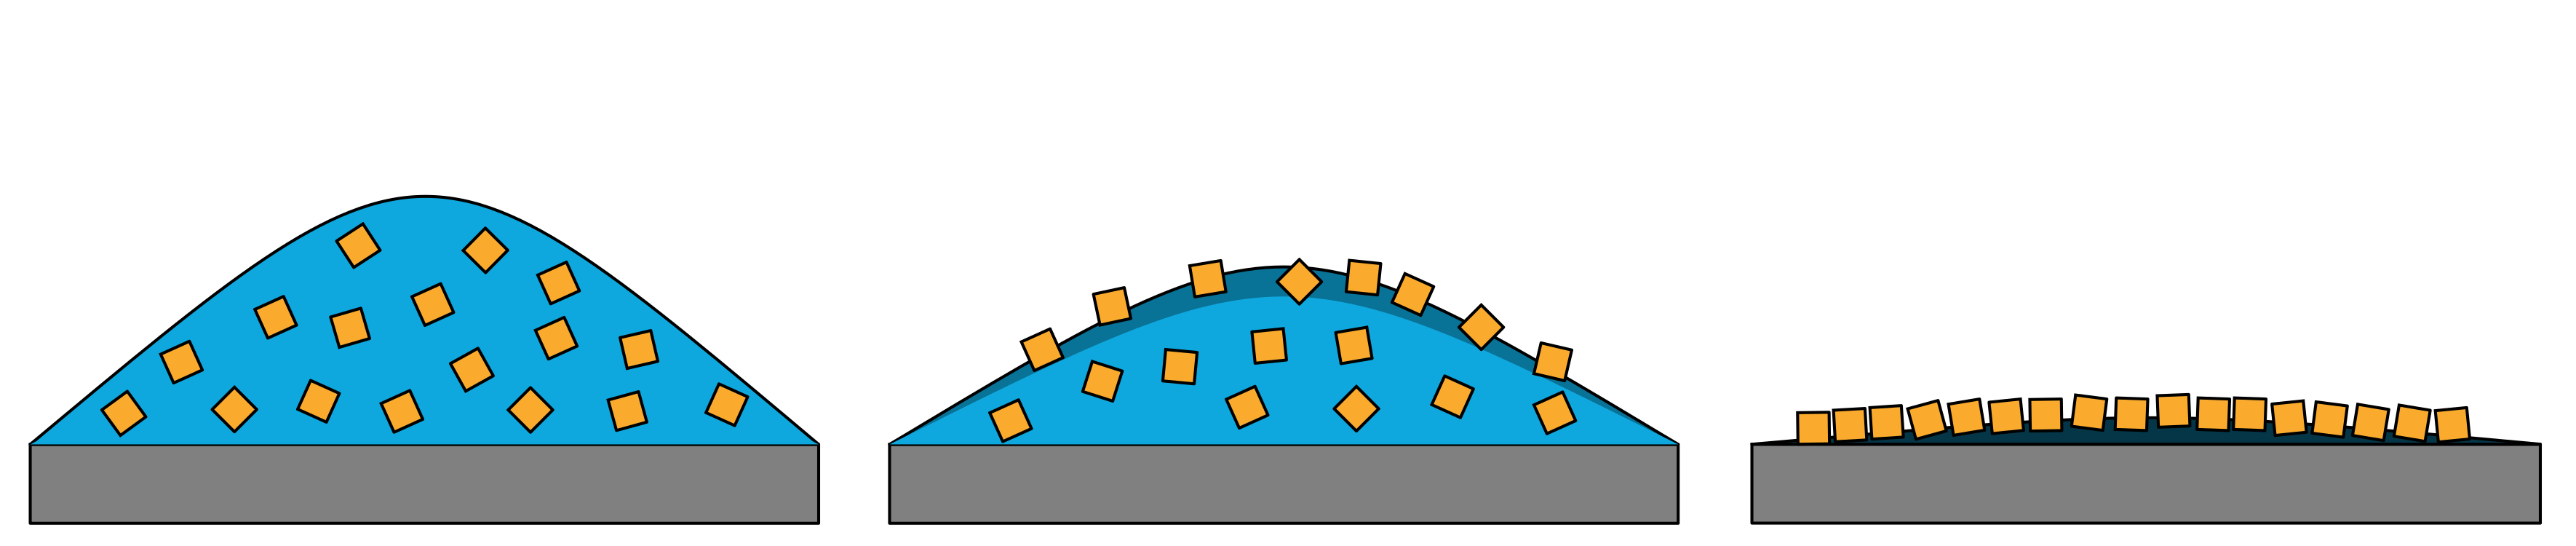
\includegraphics{monolayers_preparation_dryingStages}
    \caption{\label{fig:monolayers:preparation:dryingConditions:dryingStages} Depiction of the evolution during the first drying stage according to \cite{Bigioni_2006_Kinet}. As the droplet shrinks it fixes the nanoparticles on the droplet surface, where they can still move in two dimensions to form a long range ordered lattice. Finally the ordered structure remains with the remaining slow evaporating solvent.}
  \end{figure}

  In the drop casting method, the nanoparticles are transferred to a substrate by spreading a drop of dispersion on a flat surface and allowing the solvent to evaporate slowly, while the nanoparticles self-assemble.
  It is therefore an instrumentally cheap and a material efficient method, where the exact amount of nanoparticles needed for a monolayer on a given area is set.
  Additionally, once a monolayer has successfully been formed, the drop casting method is easily reusable to prepare multi layered samples, by repeating the process sequentially.
  The challenge of the drop casting method is to control the self-assembly process by manipulating the environmental conditions during the evaporation process and choosing the correct solvent for the nanoparticles.
  Bigioni \etal \cite{Bigioni_2006_Kinet} showed for dodecanethiol-ligated gold nanoparticles that a combination of toluene/dodecanethiol as solvent/co-solvent mixture leads to a large long-range order on the micrometer scale.
  The basic idea of the kinetic theory of Bigioni \etal is that the nanoparticles pin and self-assemble on the droplet surface as depicted in \reffig{fig:monolayers:preparation:dryingConditions:dryingStages}.
  The particles move to the surface for one, because the shrinking droplet height catches particles from the dispersion.
  And for the other, as a mechanism in the solvent reduces the diffusion constant on the droplet surface in comparison to the diffusion in the bulk droplet.
  In this work, it is attempted to reproduce this mechanism described by Bigioni for gold nanoparticles to oleic acid-ligated ferrite nanoparticles.
\end{document}